\documentclass{article}
\usepackage{graphicx} % Required for inserting images
\usepackage{kotex}
\usepackage{listings}
\usepackage{geometry}
\usepackage{xcolor}

\geometry{
    a4paper,
    left=30mm,
    right=30mm,
    top=30mm,
    bottom=40mm
}

\lstset{language=C++,
            basicstyle=\ttfamily,
            keywordstyle=\color{blue}\ttfamily,
            stringstyle=\color{red}\ttfamily,
            commentstyle=\color{teal}\ttfamily,
            numberstyle=\tiny\color{gray}\ttfamily,
            morecomment=[l][\color{magenta}]{\#}
            breakatwhitespace=false,         
            breaklines=true,                 
            captionpos=b,                    
            keepspaces=true,                 
            numbers=left,                    
            numbersep=5pt,                  
            showspaces=false,                
            showstringspaces=false,
            showtabs=false,                  
            tabsize=2
}

\title{객체지향프로그래밍 \\
\large HW02}
\author{C211123 이준선}
\date{2023년 3월 16일}

\begin{document}

\maketitle

\section{HW02}
문자열을 입력하면 알파벳 26자를 인덱스로 하여 알파벳 수를 계산하여 다음과 같이 출력하는 프로그램 작성하시오. 단, cin.getline(), isalpha(), tolower()함수를 사용한다.
(출력 생략)
\section{과제 코드}
\begin{lstlisting} [language=C++, escapeinside=``, caption=main.cpp, label={lstlisting:main.cpp}]
#include <iostream>
#include <string>
#include <unordered_map>
#include <algorithm>

class StringManager
{
public:
    StringManager() = default;
    ~StringManager() = default;

    void printMenu() const {
        std::cout << "`영문 텍스트를 입력하세요. 히스토그램을 그립니다.`" << std::endl;
        std::cout << "`텍스트의 끝은` "<< endChar << " `입니다.` " << maximumCount << "`개까지 가능합니다.`" << std::endl;
    }

    void getString() {
        std::string input;
        std::getline(std::cin, input, endChar);
        this->input = input.substr(0, maximumCount);

        for (const auto c : this->input) {
            if (std::isalpha(c)) {
                alphabetCount++;
            }
        }
    }


    auto createHistogram() {
        for (const auto c : input) {
            // if c is not alphabet, continue
            if (!std::isalpha(c)) continue;
            histogram[c]++;
        }
    }

    const auto& getHistogram() const {
        return histogram;
    }

    int getAlphabetCount() const {
        return alphabetCount;
    }

    void printHistogram() {
        for (char c = 'a'; c <= 'z'; c++) {
            _drawBar(c);
        }
    }

    void printStatus() const {
        std::cout << "`총 알파벳 수` " << getAlphabetCount() << std::endl;
    }

    void toLower() {
        for (auto& c : input) {
            c = std::tolower(c);
        }
    }

private:
    std::string input;
    int maximumCount = 10000;
    char endChar = ';';
    int alphabetCount = 0;
    std::unordered_map<char, int> histogram;

    void _drawBar(const char c) {
        std::cout << c << " (" << histogram[c] << ")\t: ";
        for (std::size_t i = 0; i < histogram[c]; i++) {
            std::cout << "*";
        }
        std::cout << std::endl;
    }
};

int main()
{
    StringManager manager;
    manager.printMenu();
    manager.getString();
    manager.toLower();
    manager.createHistogram();
    manager.printStatus();
    manager.printHistogram();

    return 0;
}
\end{lstlisting}
\section{결과}
\begin{figure}[ht]
    \centering
    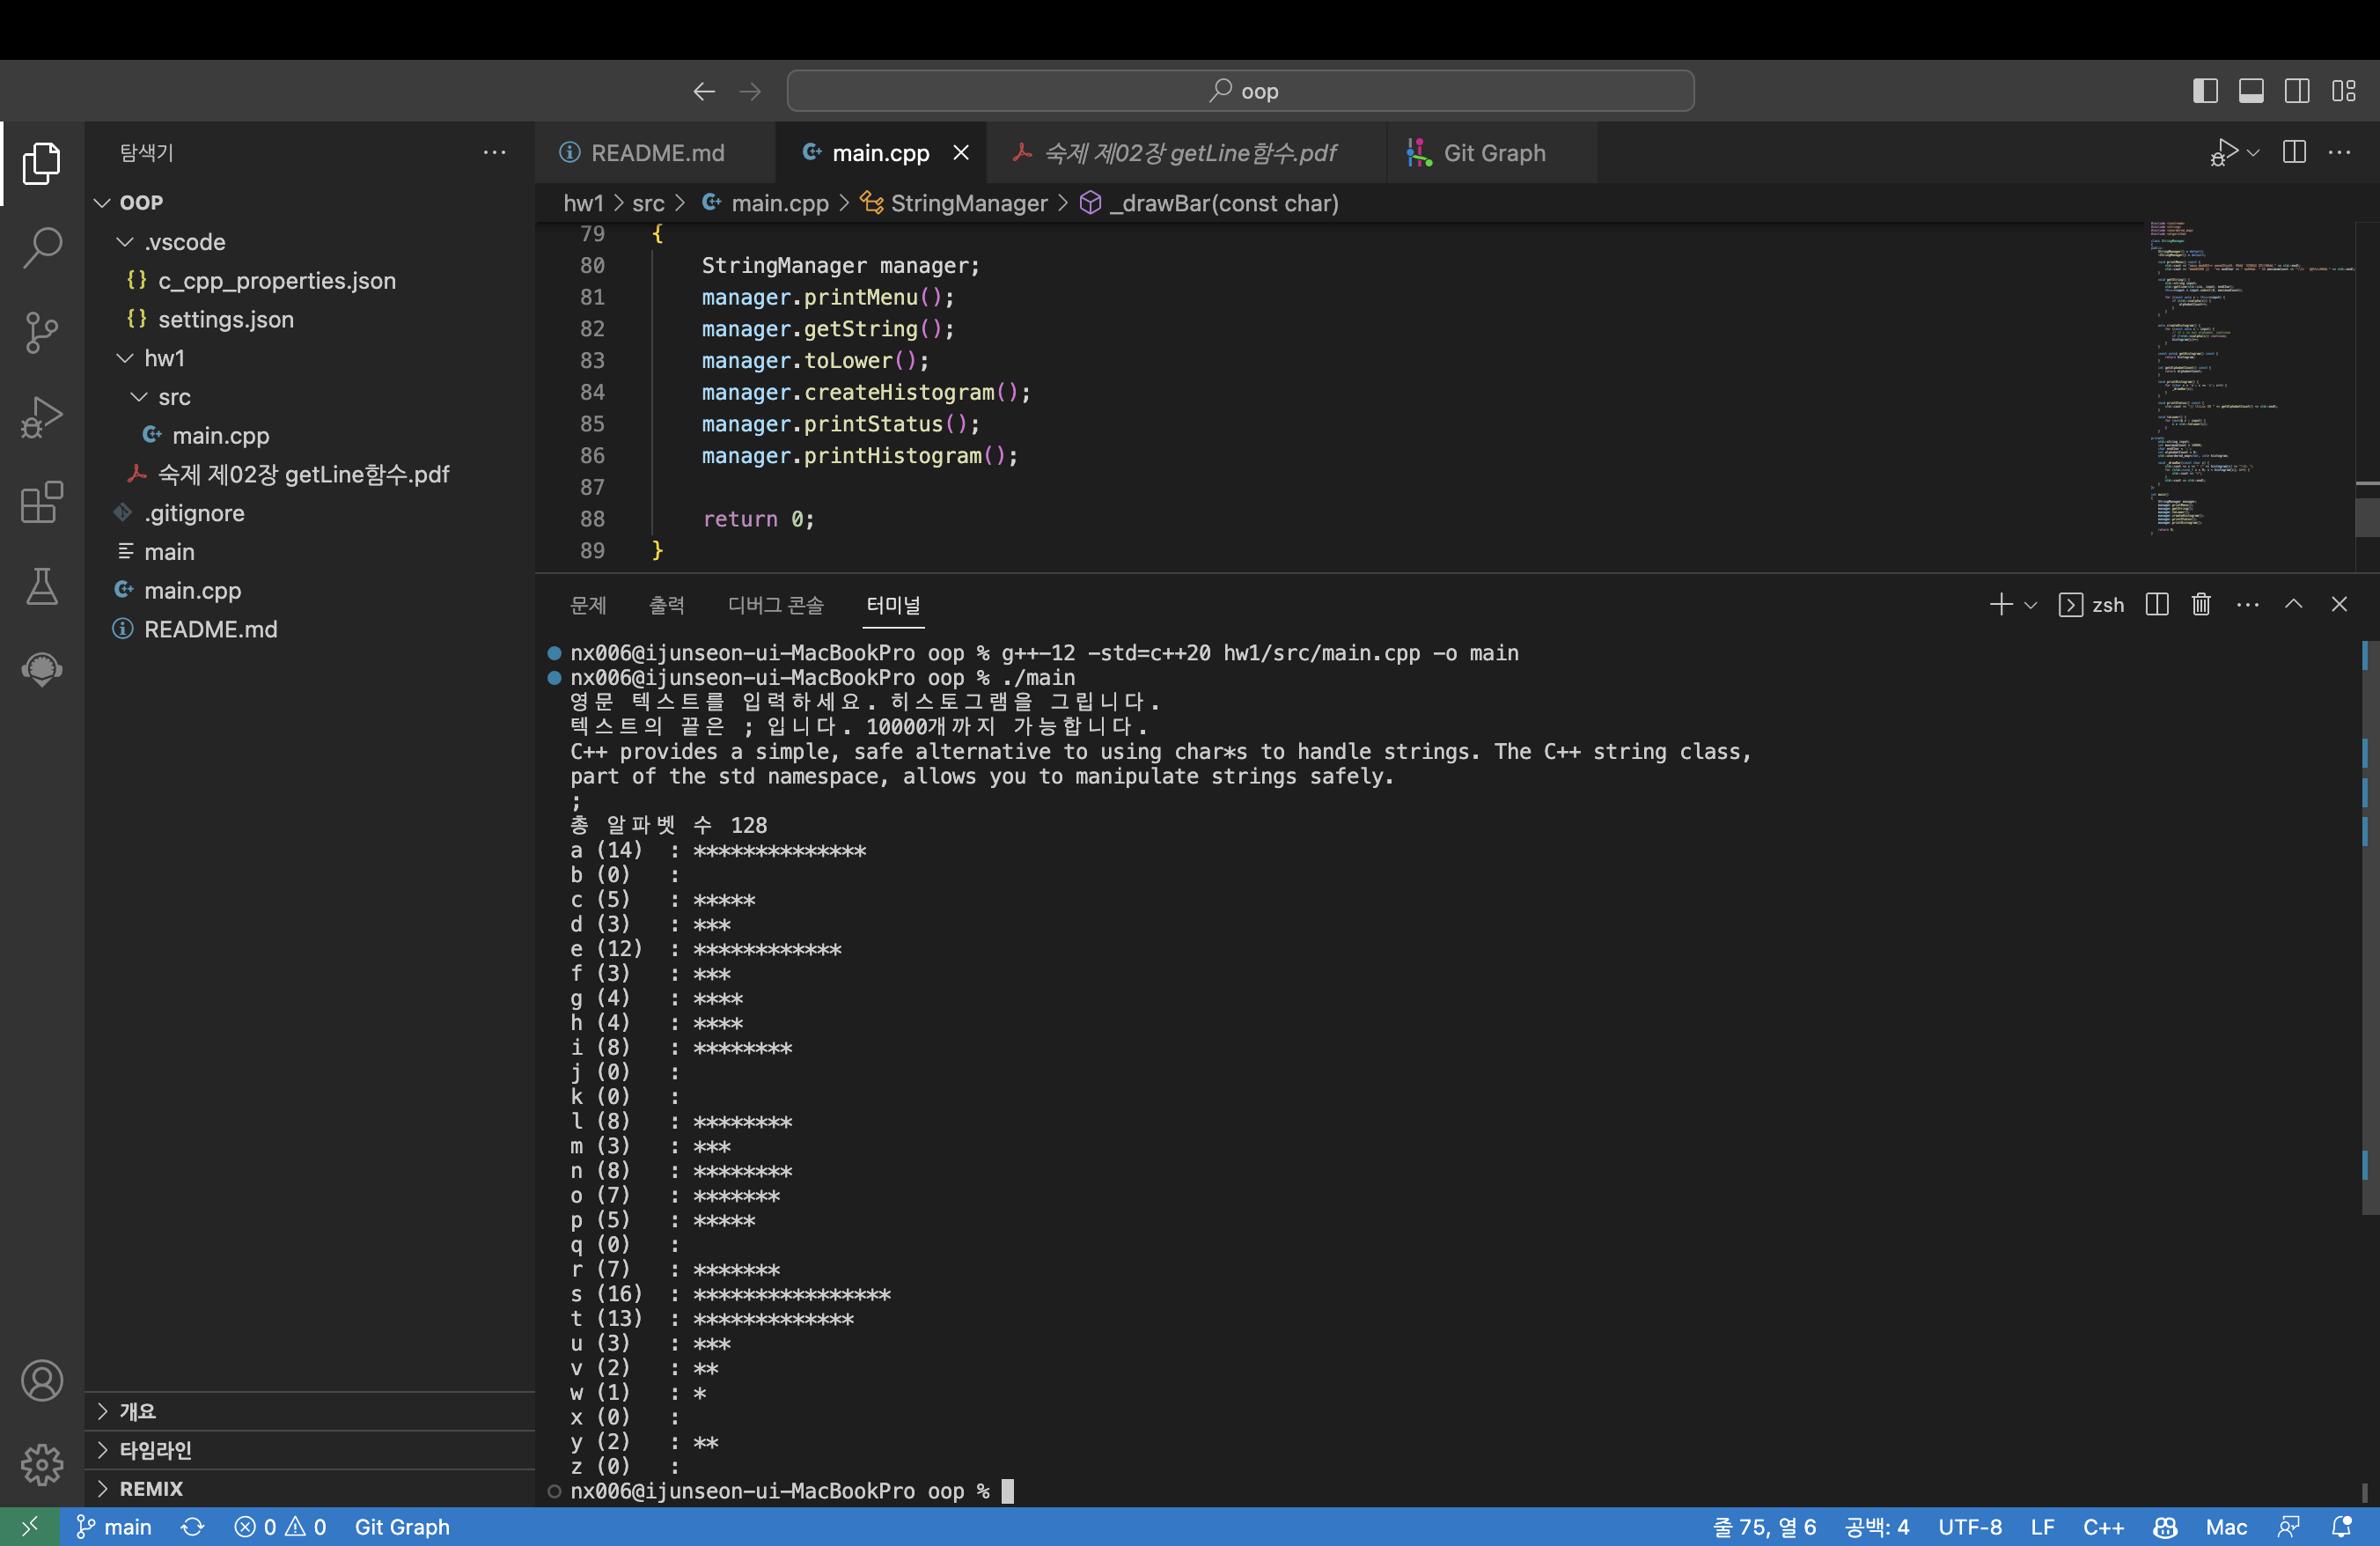
\includegraphics[width=\textwidth]{result.png}
    \caption{결과 사진}
    \label{fig:result}
\end{figure}

\section{분석}
문자열을 입력받고, 그 문자열 속에 들어있는 알파벳들 각각의 숫자를 출력하는 문제입니다.

문자열을 입력받을 때는 getline() 함수를 이용해야 한다는 조건이 존재합니다. 또한 대문자와 소문자를 구분하지 않는데, 이때 std::tolower() 함수를 이용하라고 힌트를 주고 있습니다.

문자열의 최대 입력 갯수는 10,000개까지 가능합니다.

먼저 알파벳에 대응하는 숫자를 출력해야 합니다. 이는 char $\rightarrow$ int 쌍의 해시맵을 이용할 수 있습니다. 이때 알파벳을 순서대로 출력해야 하는데, 어차피 개수가 0인 알파벳을 이용해야 하므로 굳이 삽입 및 탐색에 O(N)의 시간이 걸리는 map을 이용할 필요는 없습니다. unordered\_map을 이용하면 됩니다.

한편 오직 알파벳만 카운팅해야 합니다. 이는 isalpha 함수를 이용해야 할 것을 문제에서 힌트를 주고 있습니다.

\subsection{코드 설명}
\begin{lstlisting} [language=C++, escapeinside=``, caption=main.cpp, label={lstlisting:getstring}]
void getString() {
    std::string input;
    std::getline(std::cin, input, endChar);
    this->input = input.substr(0, maximumCount);
    for (const auto c : this->input) {
        if (std::isalpha(c)) {
            alphabetCount++;
        }
    }
}

void toLower() {
    for (auto& c : input) {
        c = std::tolower(c);
    }
}
\end{lstlisting}

문자열을 입력받는 함수입니다. std::getline 함수를 이용하고 있습니다. endChar는 ; 입니다. 이후에 만약 입력받은 문자열의 크기가 maximumCount인 10,000을 넘어가는 것을 방지하기 위해, std::string::substr 메소드를 이용해 0부터 maximumCount - 1까지 범위를 잘라서, 클래스 멤버 변수에 저장합니다.

이후에 input을 선형 탐색하면서, 만약 c가 알파벳이면 alphabetCount의 개수를 증가시킵니다.

주의해야 할 점은 문제에서의 조건이 대소문자를 구분하지 않는 것이기에, input의 모든 알파벳을 소문자로 만들어야 합니다. std::tolower을 이용하여 소문자로 바꿀 수 있고, 원본을 바꿔야 하기 때문에 참조를 써야 하는데 주의해야 합니다.

총 $O(n)$의 시간이 걸립니다.

\begin{lstlisting} [language=C++, escapeinside=``, caption=main.cpp, label={lstlisting:createHistogram}]
auto createHistogram() {
    for (const auto c : input) {
        // if c is not alphabet, continue
        if (!std::isalpha(c)) continue;
        histogram[c]++;
    }
}
\end{lstlisting}
해시맵인 히스토그램을 생성하는 함수입니다. input에 대해서 순회하며, 만약 알파벳이 아니라면 histogram을 생성하지 않고, 알파벳일 때 히스토그램을 생성합니다. 해당 알파벳을 키로 하여 value인 크기를 1씩 증가시킵니다.

\begin{lstlisting} [language=C++, escapeinside=``, caption=main.cpp, label={lstlisting:drawbar}]
void _drawBar(const char c) {
    std::cout << c << " (" << histogram[c] << ")\t: ";
    for (std::size_t i = 0; i < histogram[c]; i++) {
        std::cout << "*";
    }
    std::cout << std::endl;
}
\end{lstlisting}

히스토그램 바를 그리는 함수입니다.
\end{document}
